%%%%%%%%%%%%%%%%%%%%%%%%%%%%%%%%%%%%%%%%%%
% Short Sectioned Assignment
% LaTeX Template
% Version 1.0 (5/5/12)
%
% This template has been downloaded from:
% http://www.LaTeXTemplates.com
%
% Original author:
% Frits Wenneker (http://www.howtotex.com)
%
% License:
% CC BY-NC-SA 3.0 (http://creativecommons.org/licenses/by-nc-sa/3.0/)
%
%%%%%%%%%%%%%%%%%%%%%%%%%%%%%%%%%%%%%%%%%

%----------------------------------------------------------------------------------------
%	PACKAGES AND OTHER DOCUMENT CONFIGURATIONS
%----------------------------------------------------------------------------------------

%\documentclass[paper=a4, fontsize=11pt]{scrartcl} % A4 paper and 11pt font size
\documentclass[fontsize=11pt]{scrartcl}

\usepackage[T1]{fontenc} % Use 8-bit encoding that has 256 glyphs
\usepackage{fourier} % Use the Adobe Utopia font for the document - comment this line to return to the LaTeX default
\usepackage[english]{babel} % English language/hyphenation
\usepackage{amsmath,amsfonts,amsthm} % Math packages
\usepackage{graphicx}

\usepackage{lipsum} % Used for inserting dummy 'Lorem ipsum' text into the template

\usepackage{sectsty} % Allows customizing section commands
\allsectionsfont{\centering \normalfont\scshape} % Make all sections centered, the default font and small caps

%Make figures and all floats centered
\makeatletter
\g@addto@macro\@floatboxreset\centering
\makeatother

\usepackage{fancyhdr} % Custom headers and footers
\pagestyle{fancyplain} % Makes all pages in the document conform to the custom headers and footers
\fancyhead{} % No page header - if you want one, create it in the same way as the footers below
\fancyfoot[L]{} % Empty left footer
\fancyfoot[C]{} % Empty center footer
\fancyfoot[R]{\thepage} % Page numbering for right footer
\renewcommand{\headrulewidth}{0pt} % Remove header underlines
\renewcommand{\footrulewidth}{0pt} % Remove footer underlines
\newcommand{\vectornorm}[1]{\left|\left|#1\right|\right|}
\newcommand{\norm}[1]{\left|#1\right|}
\newcommand{\bra}[1]{\langle#1|}
\newcommand{\ket}[1]{|#1\rangle}
\setlength{\headheight}{13.6pt} % Customize the height of the header
\usepackage[mathscr]{euscript}

\numberwithin{equation}{section} % Number equations within sections (i.e. 1.1, 1.2, 2.1, 2.2 instead of 1, 2, 3, 4)
\numberwithin{figure}{section} % Number figures within sections (i.e. 1.1, 1.2, 2.1, 2.2 instead of 1, 2, 3, 4)
\numberwithin{table}{section} % Number tables within sections (i.e. 1.1, 1.2, 2.1, 2.2 instead of 1, 2, 3, 4)

%\setlength\parindent{0pt} % Removes all indentation from paragraphs - comment this line for an assignment with lots of text

%----------------------------------------------------------------------------------------
%	TITLE SECTION
%----------------------------------------------------------------------------------------

\newcommand{\horrule}[1]{\rule{\linewidth}{#1}} % Create horizontal rule command with 1 argument of height

\title{	
\normalfont \normalsize 
\textsc{Brigham Young University, Department of Physics and Astronomy} \\ [25pt] % Your university, school and/or department name(s)
\horrule{0.5pt} \\[0.4cm] % Thin top horizontal rule
\huge Effect of grid-point packing fraction on Reimann summation \\ % The assignment title
\horrule{2pt} \\[0.5cm] % Thick bottom horizontal rule
}

\author{Gus L. W. Hart} % Your name

\date{\normalsize\today} % Today's date or a custom date

\begin{document}

\maketitle % Print the title

%----------------------------------------------------------------------------------------
%	Paper Body Start
%----------------------------------------------------------------------------------------

\section{Simple Example}
Consider functions defined on the unit square that will be integrated using Riemann summation. As an
example, we will begin with $f(x,y)=\sin(\pi x)\sin(\pi y)$. This function is shown in
Fig.~\ref{fig:hump}.

The obvious way to integrate this function numerically is to partition the domain into $n\times n$
squares, evaluate the function in each square and then perform the sum: 
$$
S=\sum_{i=1}^{N_x}\sum_{j=1}^{N_y}f(x_i,y_i)\Delta x\Delta y
$$
\begin{figure}
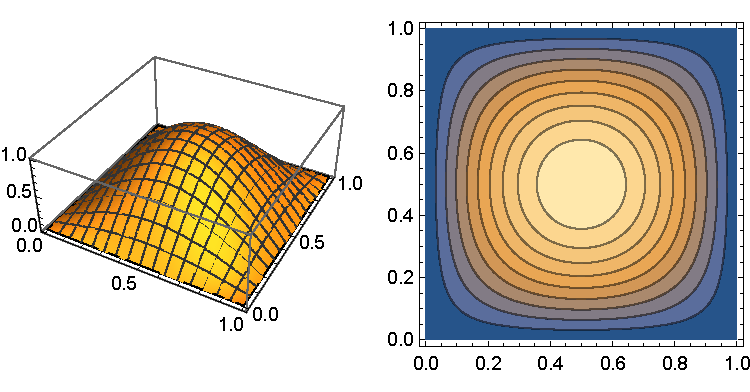
\includegraphics[width=.75\linewidth]{figs/hump.png}
\caption{Two different visualizations of the function $f(x,y)=\sin(\pi x)\sin(\pi y)$.\label{fig:hump}}
\end{figure}
Riemann summation is formally equivalent to writing the function as a Fourier series and then
integrating the series term by term (only the leading, constant term contributes a non-zero value).   
Figure \ref{fig:MPgrid} shows the simple idea of a straight-forward grid for the numerical
integration. The so-called \emph{Monkhorst-Pack} grids are the generalization of this to idea to
integration domains defined by (generally) non-orthogonal basis vectors. 

\begin{figure}
\includegraphics[width=.75\linewidth]{figs/mp_example.png}
\caption{Examples of two integration grids. Left: A function
  defined over a square domain. The integration grid points lie on surfaces of constant Cartesian
  coordinates. The integration grid ``tile'' is, except for scale, identical to the function
  domain. Right: A function defined over a rhombus and the corresponding Monkhorst-Pack-type
  grid. The integration grid is defined by lattice vectors that are not orthogonal. Again the
  integration grid tile is a scaled-down replica of the domain.\label{fig:MPgrid}}
\end{figure}

\section{Packing Fraction and non-MP grids}
In his book on lattice integration methods, Ian Sloan, makes an argument (I'll include it later
after I get the book back from the library) that the effectiveness of a particular integration grid
is related to the packing fraction of the integration points. The heart of the argument comes from
expressing the integrand as a Fourier series.

The function shown in Fig.~\ref{fig:hump} has a slowly converging Fourier series because it is not
smooth at the domain edges. Consequently, we expect that numerical integration will converge rather
slowly. Indeed, in Fig.~\ref{fig:convergence}, we see that the absolute error in the integral
decreases as $\mathcal{O}(1/N)$ where $N$ is the number of sample points. This is the convergence
rate that would be expected for a standard rectangle integration rule. (A smooth function typically
converges faster because of its rapidly converging Fourier series.)

\begin{figure}
\includegraphics[width=.75\linewidth]{figs/convergence.pdf}
\caption{Convergence of numerical integral as a function of number of sample points. The absolute
  error decrease is proportional to the number of sample points.\label{fig:convergence}}
\end{figure}

Let us examine the effect of choosing non-MP-type grids on the convergence of the numerical
integral. Imagine that each integration point is expanded to a circle until the edges of neighboring
cicles are just touching, as shown in Fig.~\ref{fig:square_packing_fraction}

\end{document}
